% Product-of-Exponentials kinematic-chain schematic for notebook 02.
% Stylized 7-joint open chain: base frame {s} -> joints theta_1..theta_7 -> ee frame {b}.
% Standalone: compiles with `lualatex poe_chain.tex`; loaded via render_tikz_file.
\documentclass[tikz,border=4pt]{standalone}
\usepackage{amsmath}
\usepackage{tikz}
\usetikzlibrary{arrows.meta,calc,decorations.markings}
\begin{document}
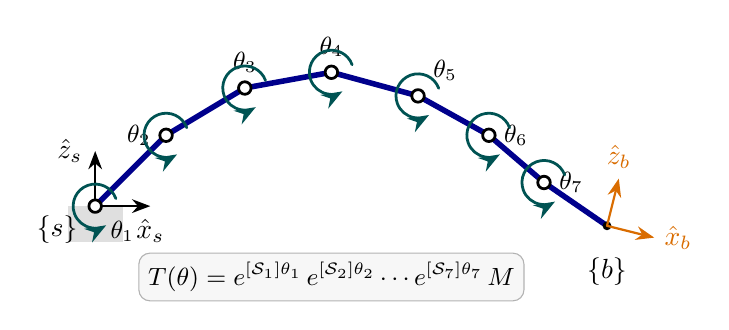
\begin{tikzpicture}[
    >=Stealth, line cap=round, line join=round, scale=1.0,
    link/.style={line width=2pt, blue!55!black},
    joint/.style={circle, draw=black, fill=white, line width=1pt, inner sep=1.6pt},
    rot/.style={->, teal!65!black, line width=1pt},
  ]
  % --- base ---
  \fill[gray!25] (-0.35,-0.45) rectangle (0.35,0.0);
  \draw[->,thick] (0,0) -- (0.7,0) node[below=1pt]{$\hat{x}_s$};
  \draw[->,thick] (0,0) -- (0,0.7) node[left=1pt]{$\hat{z}_s$};
  \node[below left] at (-0.1,0.0) {$\{s\}$};

  % --- chain vertices (stylized open chain) ---
  \coordinate (j1) at (0,0.0);
  \coordinate (j2) at (0.9,0.9);
  \coordinate (j3) at (1.9,1.5);
  \coordinate (j4) at (3.0,1.7);
  \coordinate (j5) at (4.1,1.4);
  \coordinate (j6) at (5.0,0.9);
  \coordinate (j7) at (5.7,0.3);
  \coordinate (ee) at (6.5,-0.25);

  % --- links ---
  \draw[link] (j1)--(j2)--(j3)--(j4)--(j5)--(j6)--(j7)--(ee);

  % --- joints with rotation arrows + labels ---
  \foreach \p/\lab/\dir in {%
      j1/{$\theta_1$}/below right, j2/{$\theta_2$}/left, j3/{$\theta_3$}/above,
      j4/{$\theta_4$}/above, j5/{$\theta_5$}/above right, j6/{$\theta_6$}/right,
      j7/{$\theta_7$}/right}{
    \node[joint] at (\p) {};
    \node[\dir=2pt, font=\small] at (\p) {\lab};
    \draw[rot] ([shift={(20:0.28)}]\p) arc (20:300:0.28);
  }

  % --- end-effector frame {b} ---
  \fill[black] (ee) circle (1.6pt);
  \draw[->,orange!85!black,thick] (ee) -- ($(ee)+(0.6,-0.15)$) node[right=0pt]{$\hat{x}_b$};
  \draw[->,orange!85!black,thick] (ee) -- ($(ee)+(0.15,0.6)$) node[above=0pt]{$\hat{z}_b$};
  \node[below=8pt] at (ee) {$\{b\}$};

  % --- PoE formula ---
  \node[align=center, font=\small, draw=black!30, rounded corners, fill=black!3]
       at (3.0,-0.9)
    {$T(\theta)=e^{[\mathcal{S}_1]\theta_1}\,e^{[\mathcal{S}_2]\theta_2}\cdots
      e^{[\mathcal{S}_7]\theta_7}\,M$};
\end{tikzpicture}
\end{document}
